\block{Introduction}{
	\section*{Context}
	\begin{itemize}
		\item Most of commercial transactions are still done using physical currencies
		\item Most currencies banknotes were not designed to be usable by visually impaired people
		\item Detection of counterfeit banknotes can improve the reliability of ATMs and counting machines
		\begin{itemize}
			\item Ensure proper maintenance operations
			\item Confirm value and authenticity of banknotes
		\end{itemize}
	\end{itemize}

	\begin{tikzfigure}
		\centering
		
\includegraphics[width=0.2529\linewidth]{braille}
		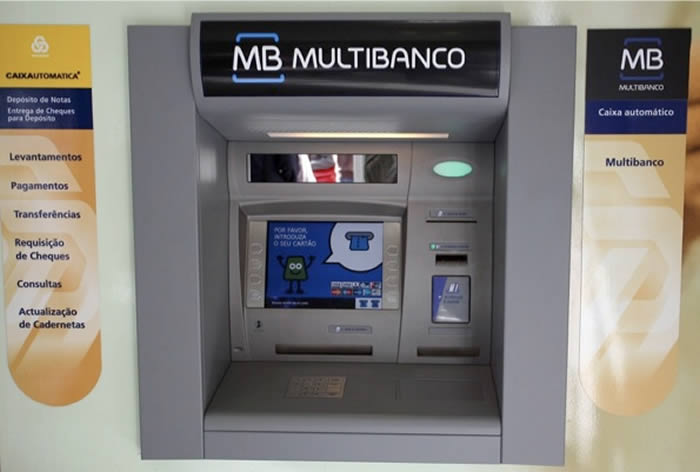
\includegraphics[width=0.2489\linewidth]{atm}
		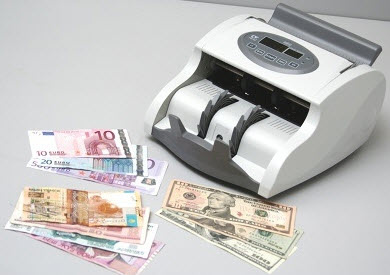
\includegraphics[width=0.2379\linewidth]{counting-machine}
		\captionof{figure}{Examples of applications of banknote recognition systems}
	\end{tikzfigure}


	\section*{Objectives}
	Implementation of a generic banknote recognition system capable of recognizing banknotes with:
	\begin{multicols}{2}
		\begin{itemize}
			\item Partial occlusions
			\item Folding
			\item Wrinkles
			\item Worn / damaged paper
			\item Multiple perspective views
			\item Multiple scales
			\item Environment clutter
			\item Variable lighting conditions
			\item Several banknotes in same image
		\end{itemize}
	\end{multicols}
}
